\documentclass[12pt]{article}
\usepackage[utf8]{inputenc}
\usepackage[russian]{babel}
\usepackage{amssymb,amsmath}
\usepackage{amsmath}
\usepackage{amsthm}
\usepackage{hyperref}
% \usepackage{biblatex}
\hypersetup{
    colorlinks,
    citecolor=black,
    filecolor=black,
    linkcolor=black,
    urlcolor=black
}
\usepackage{graphicx}
% \addbibresource{bibliography.bib}
\newtheorem{theorem}{Теорема}
\newenvironment{rowequmat}[1]{\left(\array{@{}#1@{}}}{\endarray\right)}
\textheight=24cm
\textwidth=16cm
\oddsidemargin=0pt
\topmargin=-1.5cm
\parindent=24pt
\title{Курсовой проект}
\author{\copyright Андрей Румянцев}
\date{29 ноября 2016}
\begin{document}
\begin{titlepage}
    \linespread{1.1}
    \begin{center}
    \fontsize{15pt}{15pt}\selectfont
    МИНЕСТЕРСТВО ОБРАЗОВАНИЯ РЕСПУБЛИКИ БЕЛАРУСЬ\\
    \vspace{0.5cm}
    БЕЛОРУССКИЙ ГОСУДАРСТВЕННЫЙ УНИВЕРСИТЕТ\\
    \vspace{0.5cm}
    \textit{ФАКУЛЬТЕТ ПРИКЛАДНОЙ МАТЕМАТИКИ И ИНФОРМАТИКИ}\\
    \vspace{0.5cm}
    \textit{КАФЕДРА МАТЕМАТИЧЕСКОГО МОДЕЛИРОВАНИЯ И АНАЛИЗА ДАННЫХ}\\
    \vspace{3.5cm}
    \fontsize{18pt}{18pt}\selectfont
    Румянцев\\
    Андрей Кириллович\\
    \vspace{0.5cm}
    \textbf{"Робастные оценки параметров регрессии при наличии группирования выборки"}\\
    \vspace{0.5cm}
    \fontsize{16pt}{16pt}\selectfont
    Курсовой проект\\
    \end{center}
    \vspace{3.5cm}
    \fontsize{14pt}{14pt}\selectfont
    \hspace{-0.25cm}
    \def\arraystretch{1.2}
    \begin{tabular}{l@{\hspace{3.25cm}}l}
    Допущен к защите & Научный руководитель:\\
    <<\underline{~~~~}>>~~\underline{~~~~~~~~~~~~} 2017 г&Агеева Елена Сергеевна\\
    Агеева Елена Сергеевна
    
    \end{tabular}
    \vspace{3cm}
    \begin{center}
    \fontsize{16pt}{16pt}\selectfont
    Минск, 2017
    \end{center}
  \end{titlepage}
\newpage
\tableofcontents
\newpage
\section{Введение}
Существует несколько подходов для оценки параметров регрессии, но далеко не все устойчивы к возникновениям аномальных наблюдений.
В реальной жизни аномальные наблюдения возникают постоянно, поэтому большинство методов просто неприменимо.
В прошлом веке в работах Хьюбера была заложена теория робастного оценивания.\hfill\break
Были предложены следующие робастные оценки\cite{Huber}:\hfill\break
\begin{itemize}
    \item М-Оценки\\
    \item R-Оценки\\
    \item L-Оценки
\end{itemize}
М-оценки -- некоторое подобие оценок максимального правдоподобия(ММП-оценки - частный случай), L-оценки строятся на основе линейных комбинаций порядковых статистик, R-оценки -- на основе ранговых статистик.
В данном курсовом проекте я буду моделировать функцию регрессии с аномальными наблюдениями, анализировать точность методов и находить для разных методов так называемый ''breakdown point''--процент аномальных наблюдений, при котором увеличение количества наблюдений не повысит точность методов.


\section{Теоретические сведения}
Введем линейную регрессию:\hfill\break
\begin{eqnarray}
    y_i=\beta_0+\beta_1 x_{i1}+\beta_2 x_{i2}+\dots+\beta_n x_{in}+\epsilon_i, i=\overline{1,N}
\end{eqnarray}
Или, в векторной форме:
\begin{equation}
    y_i= 
    \begin{pmatrix}
        \beta_0\\
        \beta_1\\
        \dots\\
        \beta_n
    \end{pmatrix}\times
    \begin{pmatrix}
        1\\
        x_{i1}\\
        \dots\\
        x_{in}
    \end{pmatrix}^{T}+ \epsilon_i
\end{equation}
Где $y_i$ -- $i$-е наблюдение из N наблюдений, $x_i=(x_{i1},x_{i2},\dots,x_{in})$ регрессоры, \{$\beta_k, k=\overline{0,n}$\}-- параметры регрессии, а $\epsilon_i$ -- случайная ошибка $i$-го эксперемента, распределение которой подчиняется нормальному закону с нулевым ожиданием и дисперсией $\sigma^2$.\hfill\break
В нашей задаче считаем параметры \{$\beta_k, k=\overline{0,n}$\} неизвестными, их нам и требуется найти.\hfill\break
Но мы будем рассматривать не линейную регрессию, заданную формулами (1)-(2), а линейную регрессию с аномальными наблюдениями вида:
\begin{equation}
    y_i^{\epsilon}=(\xi_i)y_i+ (1-\xi_i)\eta_i,
\end{equation}
где $\xi_i$ принимает значение, равное 1, с вероятностью $1-\widetilde{\epsilon}$ и значение, равное 0, с вероятностью $\widetilde{\epsilon}$, т.е.:
\begin{equation}
    \begin{cases}
        p(\xi_i=0)=\widetilde{\epsilon}\\
        p(\xi_i=1)=1-\widetilde{\epsilon}
    \end{cases},
\end{equation}
которая называется функцией линейной регрессии с выбросами. $\eta_i$-случайная величина из какого-то другого неизвестного нам распределения. $\widetilde{\epsilon}$ будем называть процентом аномальных наблюдений.\hfill\break
Теперь рассмотрим некоторые методы оценки параметров регрессии:
\subsection{Метод Наименьших Квадратов}
Предлоположим, что случайные ошибки подчиняются нормальному закону распределения вероятностей:
\begin{equation}
    L\{\epsilon_i\}=N_1(0,\sigma^2), i = \overline{1,n}
\end{equation}
Строим логарифмическую функцию правдоподобия. В силу (1) и (2) имеем:
\begin{equation}
    L\{y_i^{\widetilde{\epsilon}}\}=N_1(f(x_i;\theta), \sigma^2)
\end{equation}
Логарифмическая функция правдоподобия выглядит так\cite{Kharin}:
\begin{eqnarray}
    l(\theta)=\ln \prod_{i=1}^{n}(\frac{1}{\sqrt{2\pi}\sigma}e^{-\frac{(y_i^{\widetilde{\epsilon}}-f(x_i;\theta))^2}{2\sigma^2}})=-\frac{1}{2}n\ln{2\pi\sigma^2}-\frac{1}{2\sigma^2}R^2(\theta),\\
    R^2(\theta)=\sum_{i=1}^{n}(\delta y_i^{\widetilde{\epsilon}})^2=\sum_{i=1}^{n}(y_i^{\widetilde{\epsilon}}-f(x_i,\theta))^2\geq 0
\end{eqnarray}
Тогда оценка макимального правдоподобия из формул (4)-(5) такова:
\begin{eqnarray}
    \hat{\theta}=arg \min_{\theta}R^2(\theta)
\end{eqnarray}
По формулам (5)-(7) видно, что метод никак не пригоден для модели регрессии с засорениями, в чем мы далее и убедимся.

\subsection{L-оценки}
Существует способ построения устойчивых оценок, при котором для описания искажений в выборке используются распределения с ''хвостами'' более тяжелыми, чем у гипотетического распределения.
Например, используется распределение Лапласа, для которого МП-оценкой параметра ''сдвига'' является выборочная медиана, принадлежащая к классу L-оценок:
\begin{eqnarray}
    \hat{\theta}^L(x)=\sum_{t=1}^n a_tg(x_{(t)}),
\end{eqnarray}
где $x_{(1)}\leq x_{(2)} \leq \dots \leq x_{(n)}$ - вариационный ряд выборки; $g(.)$-некоторая функция, $\{a_t\}_{t=1}^n$- весовые коэффициенты.\hfill\break
Чаще всего используется частный случай (10):
\begin{eqnarray}
    \hat{\theta}^L(x)=\frac{1}{n-2q}\sum_{t=q+1}^{n-q}x_{(t)},
\end{eqnarray}
где q - наибольшее целое, не превосходящее $\alpha \cdot n (0\leq \alpha \leq \frac{1}{2})$.
При определенном выборе $\alpha$ можем получить арифметическое среднее или выборочную медиану.

\subsection{М-оценки}
Швейцарский статистик П.Хьюбер преложил использовать М-оценки\cite{Kharin}, которые являются решениями экстремальных задач вида:
\begin{eqnarray}
    \sum_{i=1}^{n}\phi(x_t;\theta)\rightarrow \min_{\theta\in \theta^{*}},
\end{eqnarray}
где $\theta^{*}$-замыкание $\theta$, $\phi(\cdot;\theta)$-некоторая функция, определяющая конкретный тип оценок и их точность.\hfill\break
Очевидно, что $\phi(\cdot;\theta)\equiv - \ln{p(\cdot;\theta)}$-обычная оценка максимального правдоподобия, построенная по модели без выбросов (1).\hfill\break
Рассмотрим теперь некоторые способы выбора $\phi(\cdot;\theta)$.\hfill\break
\subsubsection{способы выбора  функции для решения экстремальной задачи в M-оценках}
Для начала определим:
\begin{eqnarray}
    e_i=y_i^{\widetilde{\epsilon}}-(\beta_0+\beta_1 x_{i1}+\beta_2 x_{i2}+\dots+\beta_n x_{in})
\end{eqnarray}
Тогда существует такие методы\cite{RobustRegression}:\hfill\break
\begin{center}
\begin{tabular}{ |p{3cm}|p{10cm} | }
    \hline
    \multicolumn{2}{|c|}{способы выбора $\phi(\cdot;\theta)$} \\
    \hline
    Метод& Целевая функция\\
    \hline
    Метод Наименьших Квадратов&$\phi(\cdot;\theta)_{OLS}=e^2$\\
    Хьюбера&$\phi(\cdot;\theta)_{H}=
        \begin{cases}
            \frac{1}{2}e^2, |e|\leq k,\\
            k|e|-\frac{1}{2}k^2, |e|>k
        \end{cases}$\\
    Биквадратный& $\phi(\cdot;\theta)_{B}=
    \begin{cases}
        \frac{k^2}{6}(1-[1-(\frac{e}{k})^2]^3), |e|\leq k\\
        \frac{k^2}{6}, |e|>k
    \end{cases}$\\
    \hline
\end{tabular}
\end{center}
\section{моделирование функции регрессии с аномальными наблюдениями}
Для начала смоделируем функцию регрессии по методу (3). Для удобства моделируем регрессию с одним параметром x\hfill\break
Воспользуемся такими параметрами:\hfill\break
\begin{center}
\begin{tabular}{|p{5cm}|p{5cm}|}
    \hline
    Переменная&значение\\
    \hline
    Размер выборки & 1000\\
    \hline
    Процент выбросов & 10\\
    \hline
    Параметры регрессии & $(100,4)$\\
    \hline
    $x_i$ & $\sim N(-5,25)$\\
    \hline
    $\epsilon_i$&$\sim N(0,16)$\\
    \hline
    $\eta_i$&$\sim N(100,100)$\\
    \hline
\end{tabular}
\end{center}
Получаем такой график:\hfill\break
\begin{figure}[ht!]
    \centering
    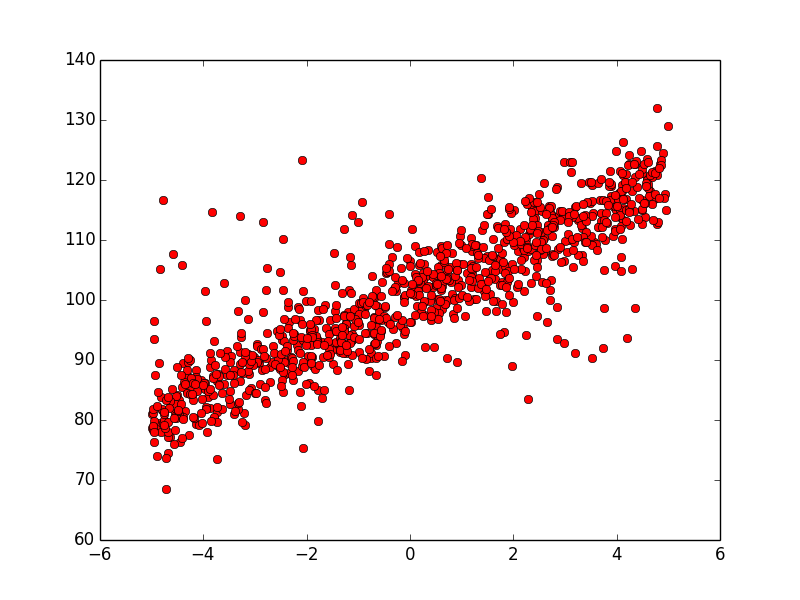
\includegraphics[width=100mm]{graphic.png}
    \caption{Вывод графика рассеяния (Y,X)\label{overflow}}
\end{figure}
\section{Поиск breakdown point у МНК и М-оценок}
Для поиска того процента загрязнений, при котором увеличение количества элементов выборки не повышает точности метода будем делать так:\hfill\break
\begin{itemize}
    \item Организуем цикл по процентам загрязнений $\widetilde{\epsilon}$\\
    \item На каждой итерации будем 20 раз моделировать выборку с $N_1=1000$ и $N_2=3000$ наблюдений.
        \begin{itemize}
            \item На каждой такой итерации суммируем невязку с точными значениями параметров для каждого количества элементов:
        \end{itemize}
    \item после цикла делим на количество суммирования каждую из сумм невязок, т.е. вычисляем такие значения:
            \begin{eqnarray}
                \widetilde{e_1^{\widetilde{\epsilon}_i}}= \frac{1}{20}\sum_{k=1}^{20}(\sum_{i=0}^{n}(\beta_i-\hat{\beta_{N_1ki}})^2)^{\frac{1}{2}}\\
                \widetilde{e_2^{\widetilde{\epsilon}_i}}= \frac{1}{20}\sum_{k=1}^{20}(\sum_{i=0}^{n}(\beta_i-\hat{\beta_{N_2ki}})^2)^{\frac{1}{2}}
            \end{eqnarray}\\
    \item если полученная усредненная невязка при 1000 наблюдений меньше либо равна невязке при 3000 наблюдений, то заканчиваем цикл - нашли breakdown point, т.е.:
            \begin{eqnarray}
                br_p=
                \begin{cases}
                    \widetilde{\epsilon_i}, if~ \widetilde{e_1^{\widetilde{\epsilon}_i}}<\widetilde{e_2^{\widetilde{\epsilon}_i}}
                \end{cases}
            \end{eqnarray}\\
    \item иначе повышаем процент на 1 и повторяем цикл: ~$\widetilde{\epsilon_{i+1}}=\widetilde{\epsilon_{i}}+1$
\end{itemize}
Такие тесты проведем для МНК и М-оценок.\hfill\break
Замечания:\hfill\break
\begin{itemize}
    \item Мы могли бы моделировать не 20 раз , а значительно больше, тем самым мы уменьшаем зависимость результата работы метода он моделируемой выборки.\\
    \item Аналогично можно заключить и для размера выборок(отношение моделируемых количеств можно значительно увеличить)
\end{itemize}
\section{Результаты программы}
\begin{center}
\begin{tabular}{|p{8cm}|p{3cm}|}
    \hline
    Метод&breakpoint\\
    \hline
    МНК & 7\%\\
    М-оценка с функцией Хьюбера& 23\%\\
    \hline
\end{tabular}
\end{center}
Итак, видим, что М-оценки  значительно устойчивее к выбросам чем МНК.\hfill\break 
\newpage
Консольный вывод программы, где показываются усредненные невязки для разных методов при $N_1=1000$ и $N_2=3000$ наблюдений соответственно:
\begin{figure}[ht!]
    \centering
    \includegraphics[width=100mm]{RLMDisperancies.png}
    \caption{Невязки М-оценок с функцией Хьюбера\label{overflow}}
\end{figure}
\begin{figure}[ht!]
    \centering
    \includegraphics[width=100mm]{OLSDisperancies.png}
    \caption{Невязки МНК\label{overflow}}
\end{figure}
\newpage
\section{Заключение}
По консольному выводу можно заметить, как растет невязка у обоих методов и при этом уменьшается расхождение невязок при увеличении объема выборки, когда процент аномальных наблюдений растет.
\newpage
% \section{Список литературы}
% \printbibliography
\begin{thebibliography}{9}
    \bibitem{Huber}
    Хьюбер Дж П.,
    \textit{Робастность в статистике:пер. с англ.}.
    М.:Мир,1984-304с

    \bibitem{Kharin}
    Харин Ю.С., Зуев Н.М., Жук Е.Е,
    \textit{Теория вероятностей, математическая и прикладная статистика: учебник}
    Минск: БГУ, 2011.-463с

    \bibitem{RobustRegression}
    John Fox \& Sanford Weisberg,
    \textit{Robust Regression},
    October 8, 2013

    \bibitem{RobustPolynomialEstimation}
    А.В. Омельченко,
    \textit{Робастное оценивание параметров полиномиальной регрессии второго порядка,}
    Харьковский национальный университет радиоэлектроники, Украина, 2009
\end{thebibliography}
\end{document}